\documentclass{beamer}

\usepackage{../macros}

\title{Graph}

\newcommand{\ANAR}{\href{https://www.spoj.com/problems/ANARC08G/}{ANARC08G}}
\newcommand{\PARADOX}{\href{https://www.spoj.com/problems/PARADOX/}{PARADOX}}

\usetikzlibrary {positioning,arrows}
\begin{document}

\frame{
  \titlepage
}



\begin{frame}[fragile]
  \frametitle{\ANAR{} - Think I will Buy Me a Football Team}

  \begin{block}{Graph Definition}
    \begin{itemize}
    \item Each bank is represented as a node.
    \item Each debt is represented as an arc beetween two nodes labeled with the debt amount.
    \end{itemize}
  \end{block}


  \begin{exampleblock}{Questions}
    \begin{itemize}
    \item How can you compute the total amount of money needed to settle all debts between the banks?
    \item How can you reduce this total amount?  
    \end{itemize}
  \end{exampleblock}

\end{frame}




\begin{frame}[fragile]
  \frametitle{\ANAR{} - Transitivity Reduction Rule}


  
\begin{columns}[t]
\begin{column}{0.48\textwidth}
  \begin{block}{Transitivity Reduction Rule}
\begin{tikzpicture}[shorten >=1pt, auto, node distance=2cm, thick,
  state/.style={circle},
  edge_style/.style={draw=black, thick}]
  \node[state] (A) at (0, 0) {$A$};
  \node[state] (B) at (1.5, 1.5) {$B$};
  \node[state] (C) at (3, 0) {$C$};
  \draw[thick,->]  (A) to node[midway] {$x$} (B)  ;
  \draw[thick,->]  (B) to node[midway] {$y$} (C);
\end{tikzpicture}


\end{block}

\end{column}
\begin{column}{0.48\textwidth}
  \begin{alertblock}{Question}
    The current flow is $x+y$. \\
    \alert{How can you reduce the flow?}
  \end{alertblock}

  \begin{block}<2>{Answer}
    The flow is reduced to $\max(x,y)$. \\
  \end{block}

\end{column}
\end{columns}

  
\begin{columns}[t]
  \begin{column}{0.48\textwidth}
    \begin{block}<2>{$y \geq x$}
      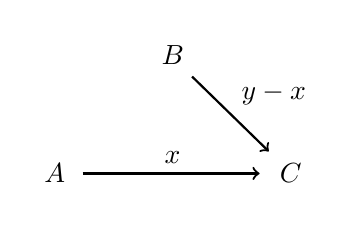
\begin{tikzpicture}[shorten >=1pt, auto, node distance=2cm, thick,
        state/.style={circle},
        edge_style/.style={draw=black, thick}]
        \node[state] (A) at (0, 0) {$A$};
        \node[state] (B) at (1.5, 1.5) {$B$};
        \node[state] (C) at (3, 0) {$C$};
        \draw[thick,->]  (A) to node[midway] {$x$} (C)  ;
        \draw[thick,->]  (B) to node[midway] {$y-x$} (C);
      \end{tikzpicture}
    \end{block}
  \end{column}
  \begin{column}{0.48\textwidth}
    \begin{block}<2>{$y \leq x$}
      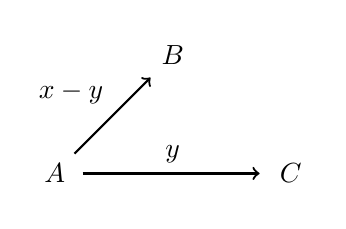
\begin{tikzpicture}[shorten >=1pt, auto, node distance=2cm, thick,
        state/.style={circle},
        edge_style/.style={draw=black, thick}]
        \node[state] (A) at (0, 0) {$A$};
        \node[state] (B) at (1.5, 1.5) {$B$};
        \node[state] (C) at (3, 0) {$C$};
        \draw[thick,->]  (A) to node[midway] {$x-y$} (B)  ;
        \draw[thick,->]  (A) to node[midway] {$y$} (C);
      \end{tikzpicture}
    \end{block}
  \end{column}

\end{columns}

\end{frame}


\begin{frame}[fragile]
  \frametitle{\ANAR{} - Fixpoint algorithm}

  \begin{alertblock}{Fixpoint Algorithm}
    Apply repeatedly the transitivity reduction rule on the graph until it is not possible. 
  \end{alertblock}


  \begin{exampleblock}{Questions}
    \begin{itemize}
    \item What is the complexity of the fixpoint algorithm?
    \item Which properties are satisfied by the graph when the fixpoint has been reached? 
    \item Is the resulting graph unique?
    \item Can you propose better algorithm that solves the problem? What is its complexity?
    \end{itemize}
  \end{exampleblock}

\end{frame}



\end{document}

%%% Local Variables:
%%% mode: latex
%%% TeX-master: t
%%% End:
